\begin{frame}
\frametitle{About This Work...}

\emph{Probabilistic Threshold $k$ Nearest Neighbor Queries over Moving Objects in Symbolic Indoor Space}.~\cite{DBLP:conf/edbt/YangLJ10} \\
B.~Yang, H.~Lu, and C.~S. Jensen.\\~\\

\begin{itemize}
  \item Published in year 2010 at the \emph{EDBT} conference.
  \item \conceptbf{Minimal Indoor Walking Distance}(MIWD) along with algorithms and data structures are proposed for distance computing and storage.
  \item Effective object indexing structures, also capture the uncertainty of object locations.
  \item On this foundation, Probabilistic threshold $k$NN (PT$k$NN) query is studied.
\end{itemize}

\end{frame}
%------------------------------------------------

\begin{frame}
\frametitle{Motivation}

\begin{itemize}
  \item Indoor positioning makes it possible to support interesting queries over large populations of moving objects.\cite{jensen2010indoor}
    \begin{itemize}
      \item shopping mall, airports, office buildings
      \item $k$NN queries over indoor moving objects enables the detection of approaching potential threats at sensitive locations in a subway system
    \end{itemize}

  \item Existing $k$NN techniques in spatial and spatiotemporal databases are inapplicable in indoor spaces.
    \begin{itemize}
      \item complex entities and topologies
      \item indoor positioning techniques differ fundamentally from outdoor GPS, low sampling frequency and accuracy
    \end{itemize}
\end{itemize}

\end{frame}
%------------------------------------------------

\begin{frame}
\frametitle{Minimal Indoor Walking Distance}

\conceptbf{Minimal Indoor Walking Distance}(MIWD) is used as the distance metric in indoor spaces.
\pause

The mapping ${Rooms}$ determines the room of an indoor position:
\pause
\begin{equation}
{Rooms: positions \rightarrow \Sigma_{rooms}}
\end{equation}

\pause

The mapping ${Doors}$ maps a room to the doors that connect the room to an adjacent room:
\pause
\begin{equation}
{Doors: \Sigma_{rooms} \rightarrow 2^{\Sigma_{doors}}}
\end{equation}

\end{frame}

%------------------------------------------------

\begin{frame}
\frametitle{Minimal Indoor Walking Distance}

\begin{columns}[c]
  \column{.52\textwidth}
  \begin{figure}[tb]
    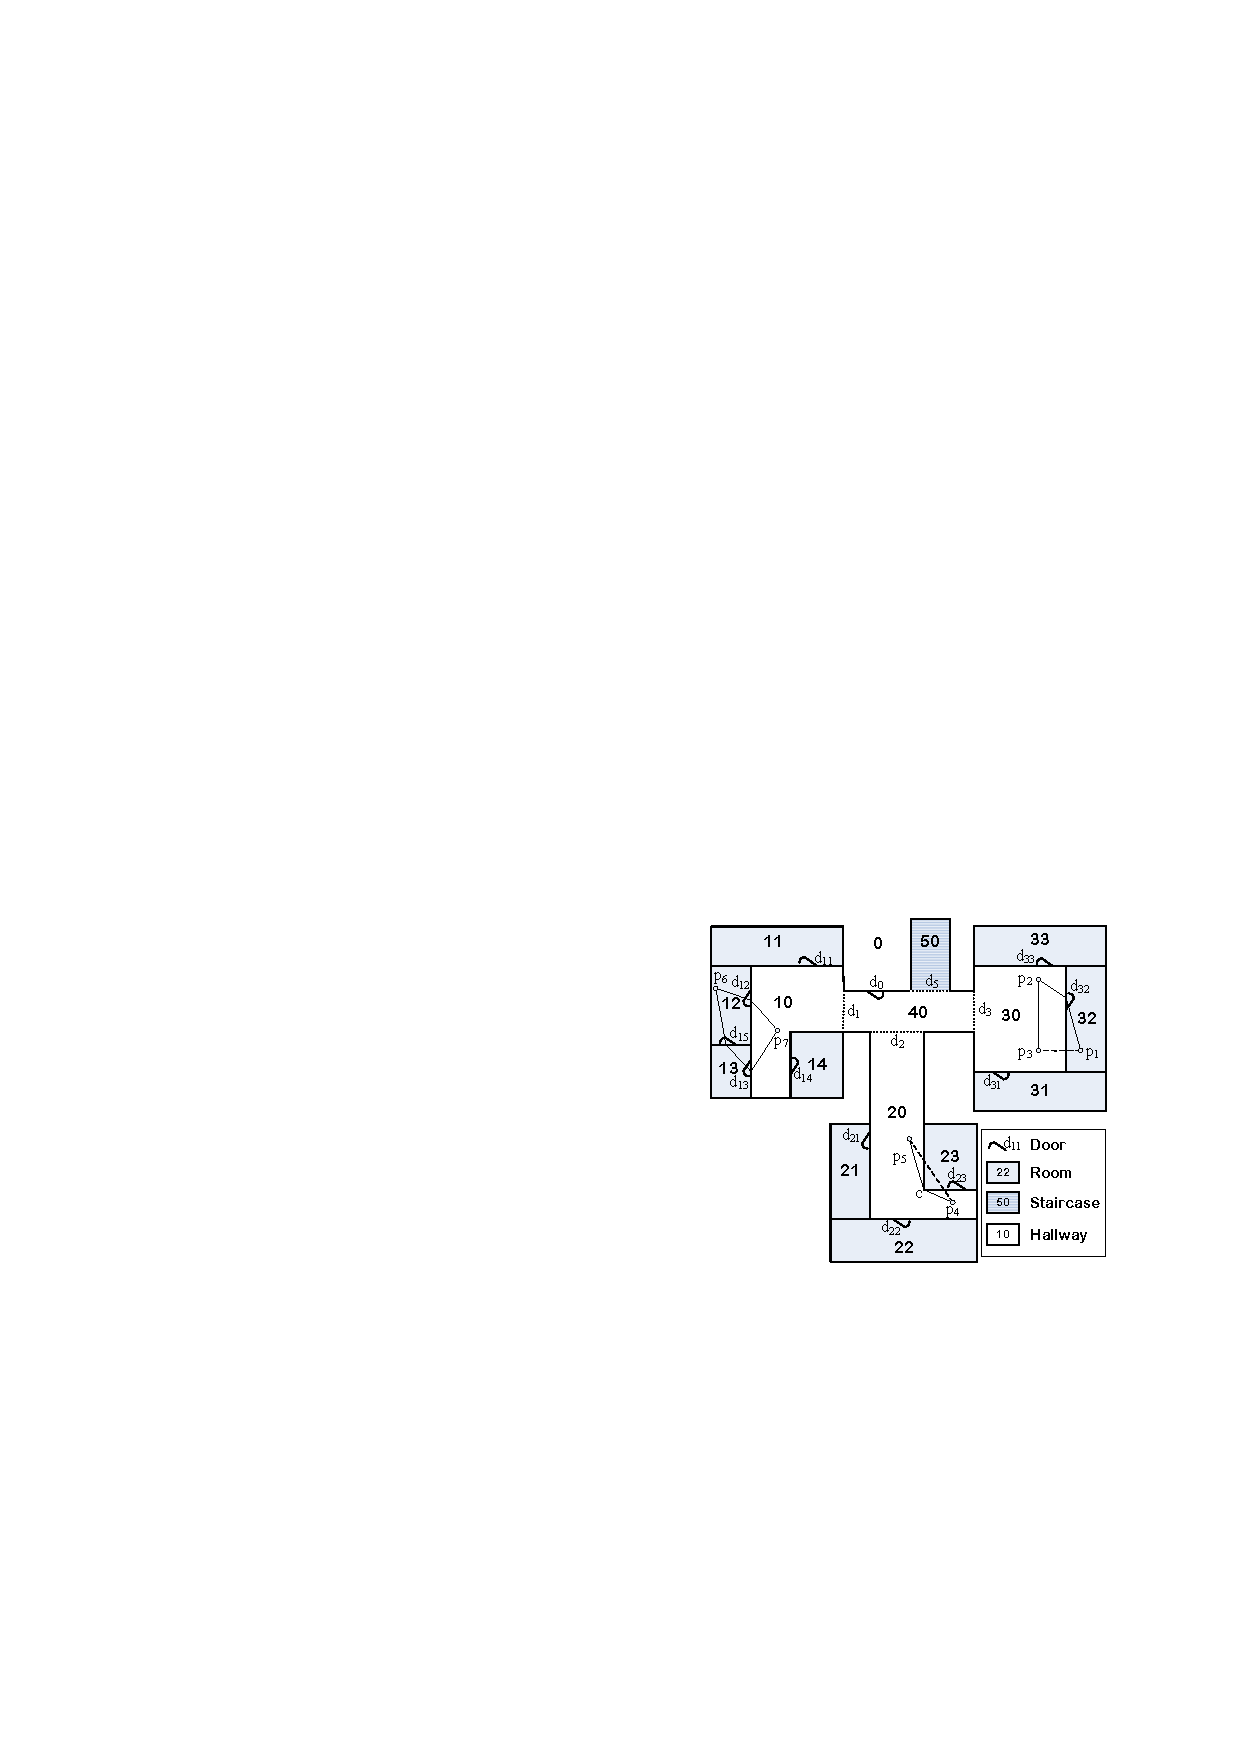
\includegraphics[width=\columnwidth]{figures/2-3/2-3-1.pdf}
  \end{figure}

  \column{.48\textwidth}
  \begin{itemize}
    \ssize{
    \item intra-room obstructed distance, termed as ${d_o}$. E.g., ${d_o(p_2, p_3) = |p_2p_3|}$ and ${d_o(p_4, p_5) = |p_4c|+|cp_5|}$.
    \item if in different rooms, it should take into account the doors connecting the rooms. E.g., ${d_{MIN}(p_1, p_2) = |p_1d_{32}| + |d_{17}p_9|}$.
    \item if there exist several paths, the correct path should be the shortest one. E.g., ${d_{MIN}(p_6, p_7) = |p_6d_{12}| + |d_{12}p_7|}$ ${\neq |p_6d_{15}| + |d_{15}d_{13}| + |d_{13}p_7|}$.
    }
  \end{itemize}

\end{columns}

\end{frame}

%------------------------------------------------

\begin{frame}
\frametitle{Minimal Indoor Walking Distance}

\conceptbf{Doors Graph} is capable of retrieving the connecting doors between two rooms, which is convenient for computing MIWD.

\begin{columns}[c]

  \column{.48\textwidth}
    \begin{figure}[tb]
      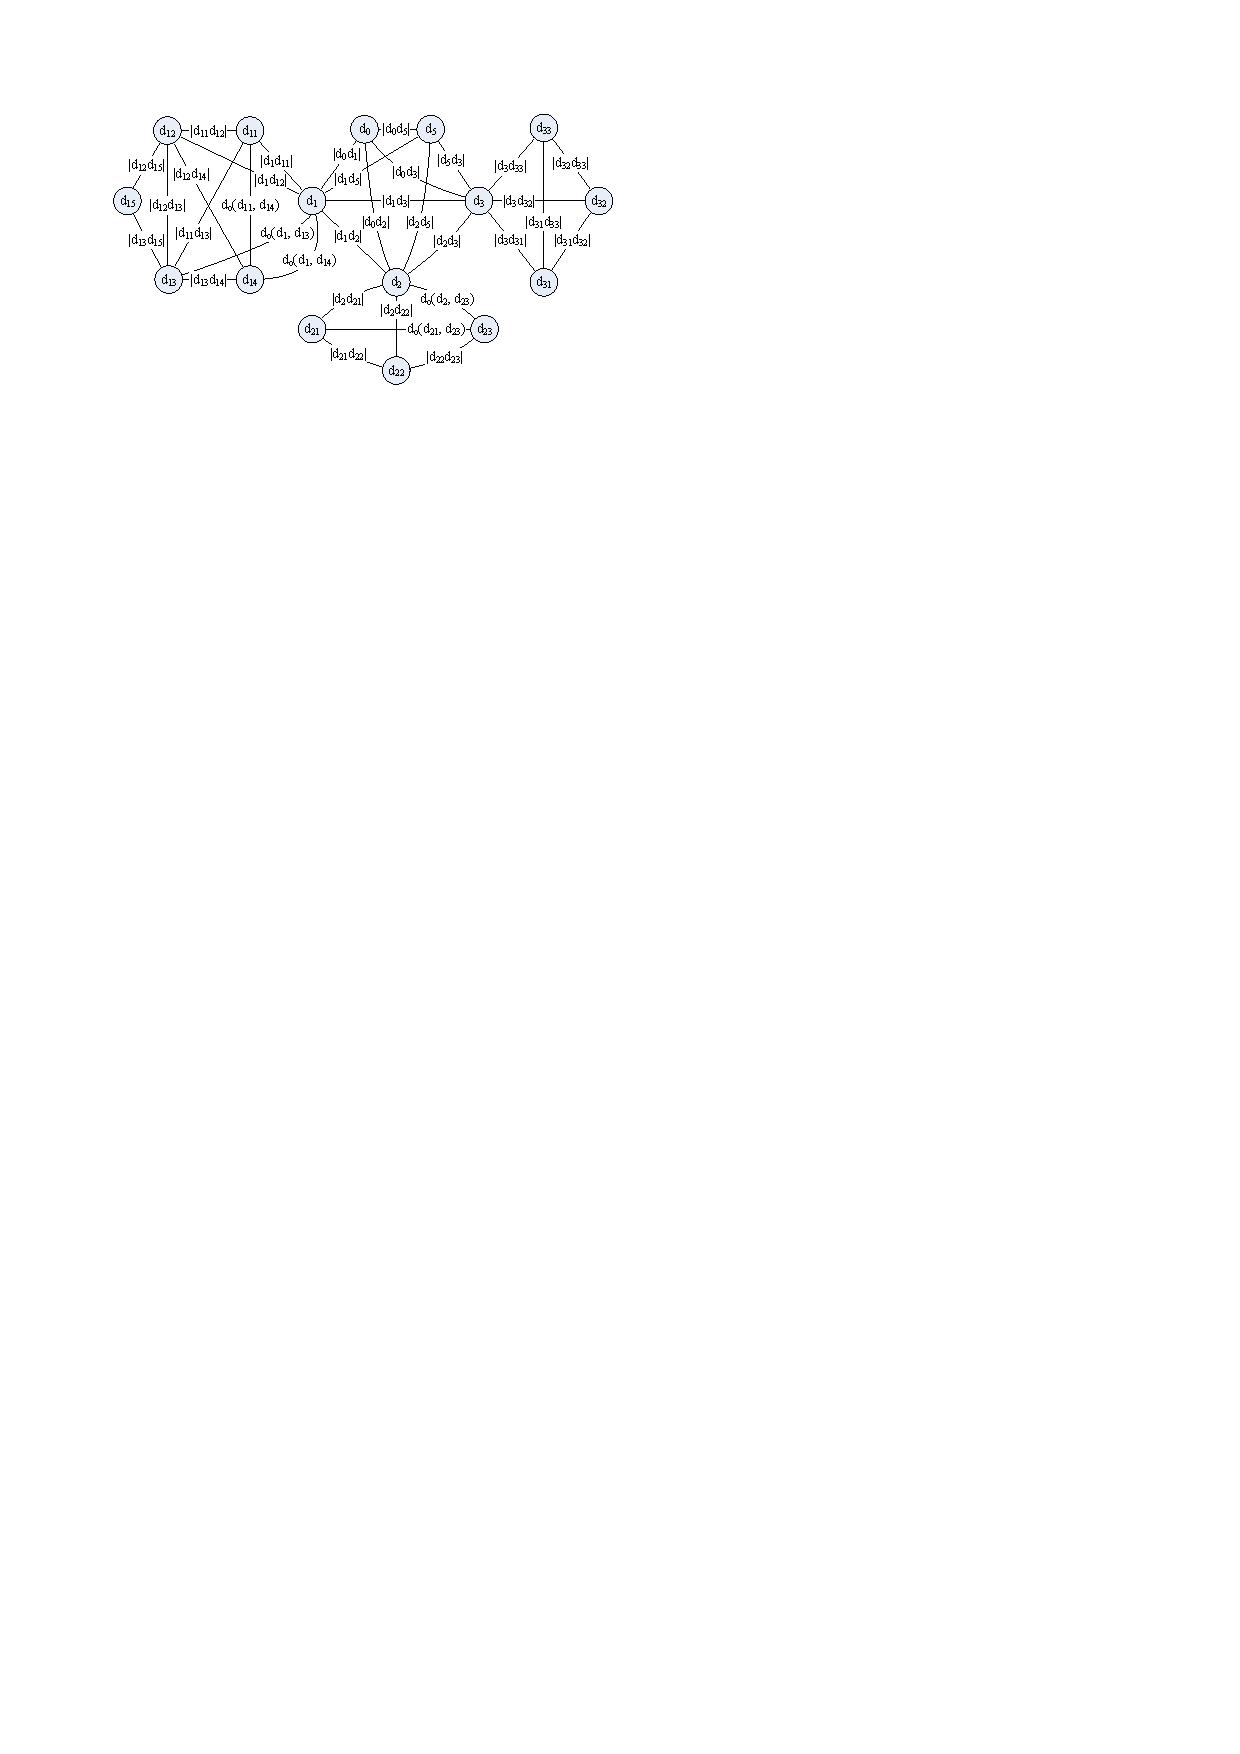
\includegraphics[width=\columnwidth]{figures/2-3/2-3-2.pdf}
    \end{figure}

  \column{.52\textwidth}
    \begin{block}{Doors Graph}
      \textrm{
      \fsize{
      \begin{itemize}
        \item ${G_{d} = \{ D, E, l_{weight} \}}$
        \item ${D = \Sigma_{doors}}$ is the set of the vertices
        \item ${E}$: An edge ${\{ d_i, d_j \}}$ exists if a room ${rm}$ exists in ${\Sigma_{rooms}}$ such that ${\{ d_i, d_j \} \subseteq Doors(rm)}$
        \item ${l_{weight}: E \rightarrow R}$ assigns to an edge the obstructed distance between the two doors as ${d_o(d_i, d_j)}$
      \end{itemize}
      }
      }
    \end{block}

\end{columns}

\end{frame}

%------------------------------------------------

\begin{frame}
\frametitle{Minimal Indoor Walking Distance}

All \conceptbf{door-to-door shortest path distances} can be computed and recorded in a hash table $\mathrm{D2D}$ according to the Doors Graph.
\pause
\begin{equation}
  \mathrm{D2D}: { \{ (d_p, d_j) \} \rightarrow R, ~~d_p, d_q \in \Sigma_{doors} }.
\end{equation}
\pause
Consequently, for two positions ${p}$ and ${q}$ in different rooms.
\pause
\begin{equation}
  {d_{MIN}(d_p, d_q) = d_o(p, d_p) + \mathrm{D2D}(d_p, d_q) + d_o(d_q, q)}
\end{equation}
where ${d_p(d_q)}$ ranges over all doors of room ${p(q)}$.
\pause
\begin{columns}[c]

  \column{.48\textwidth}
    \begin{figure}[tb]
      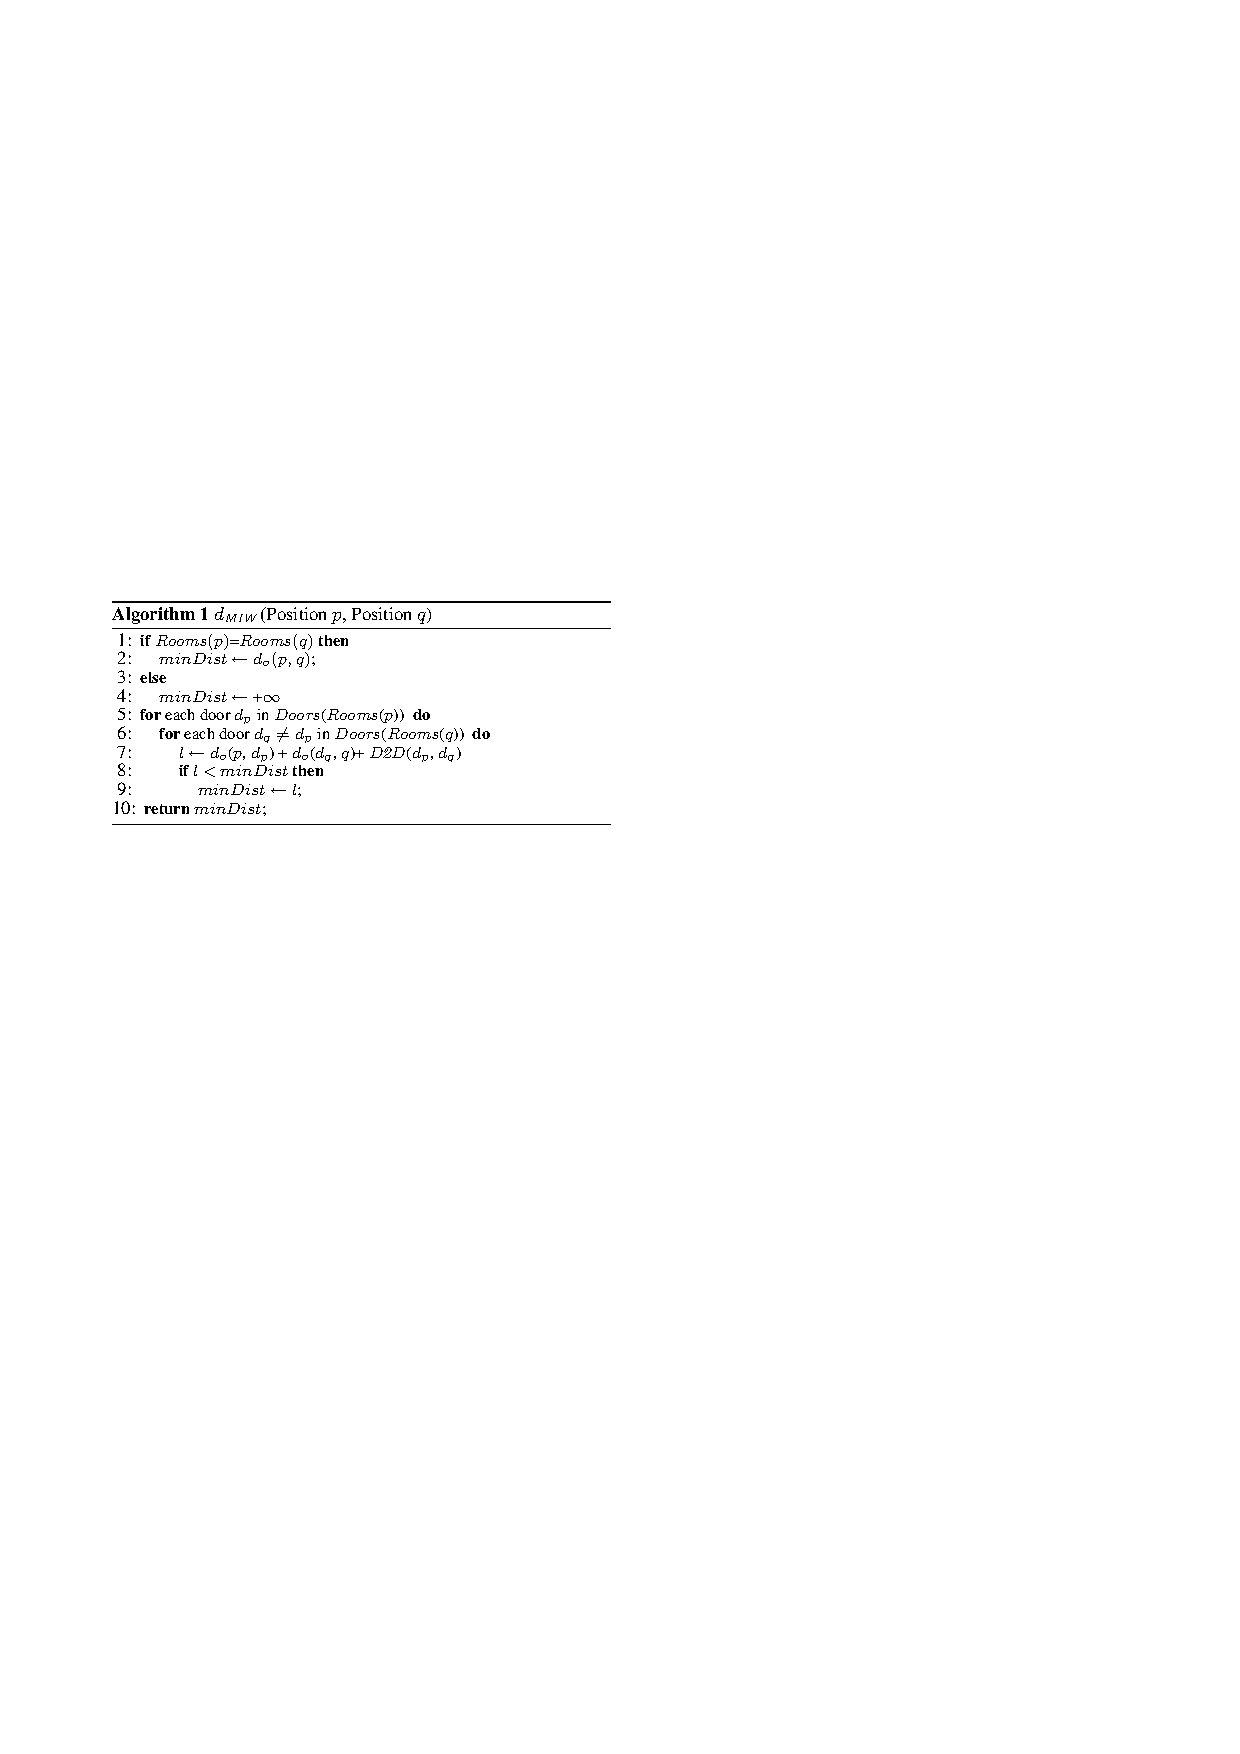
\includegraphics[width=\columnwidth]{figures/2-3/2-3-3.pdf}
    \end{figure}

  \column{.52\textwidth}
    \ssize{
    it is possible to adapt this notion of distance to accommodate other semantics. For example, a person might prefer a longer indoor path that passes as few doors as possible.
    }

\end{columns}

\end{frame}

%------------------------------------------------

\begin{frame}
\frametitle{Symbolic Indoor Positioning}

  each device detects and reports the observed objects at a relatively high sampling rate.\\~

  A reading ${(deviceID, objectID, t)}$ states that object ${objectID}$ is detected by device ${objectID}$ at time ${t}$.\\~

  Only its first and last appearances in a device's range are of interest.\\~

  \begin{fitemize}
    \item ${flag = ENTER}$ indicates that the object is entering the device's activation range
    \item ${flag = LEAVE}$ indicates that the object is leaving the device's activation range
  \end{fitemize}

\end{frame}

%------------------------------------------------

\begin{frame}
\frametitle{Positioning Devices Deployment Graph~\cite{DBLP:conf/cikm/YangLJ09}}

\begin{columns}[c]

  \column{.57\textwidth}
  \begin{itemize}
    \fsize{
    %\item More advanced compared to \emph{RFID Deployment Graph}.
    \item Two types of positioning devices
      \begin{itemize}
        \ssize{
        \item Partitioning Device -- \emph{undirected} (\conceptbf{UP}), e.g., ${d_{21}}$ -- \emph{directed} (\conceptbf{DP}), e.g., ${d_{11}}$ and ${d_{11'}}$
        \item Presence Device -- (\conceptbf{PR})
        }
      \end{itemize}
    \item Note an indoor space is partitioned into \emph{activation ranges} and \emph{cells}
    }
  \end{itemize}
  \begin{block}{Deployment Graph}
    \textrm{
    \begin{itemize}
      \ssize{
      \item ${G = \{C, E, \Sigma_{devices}, l_E\}}$
      \item ${C}$: the set of cells
      \item ${E}$: the set of edges, ${\{ c_i, c_j \}}$ where ${c_i, c_j \in C}$
      \item ${\Sigma_{devices}}$: a mapping from ${deviceID}$ to activation range and type
      \item ${l_E}$ maps an edge to a set of positioning devices, i.e., ${E \rightarrow 2^{\Sigma_{devices}}}$
      }
    \end{itemize}
    }
  \end{block}

  \column{.43\textwidth}
    \vspace{-30pt}
    \begin{figure}[tb]
      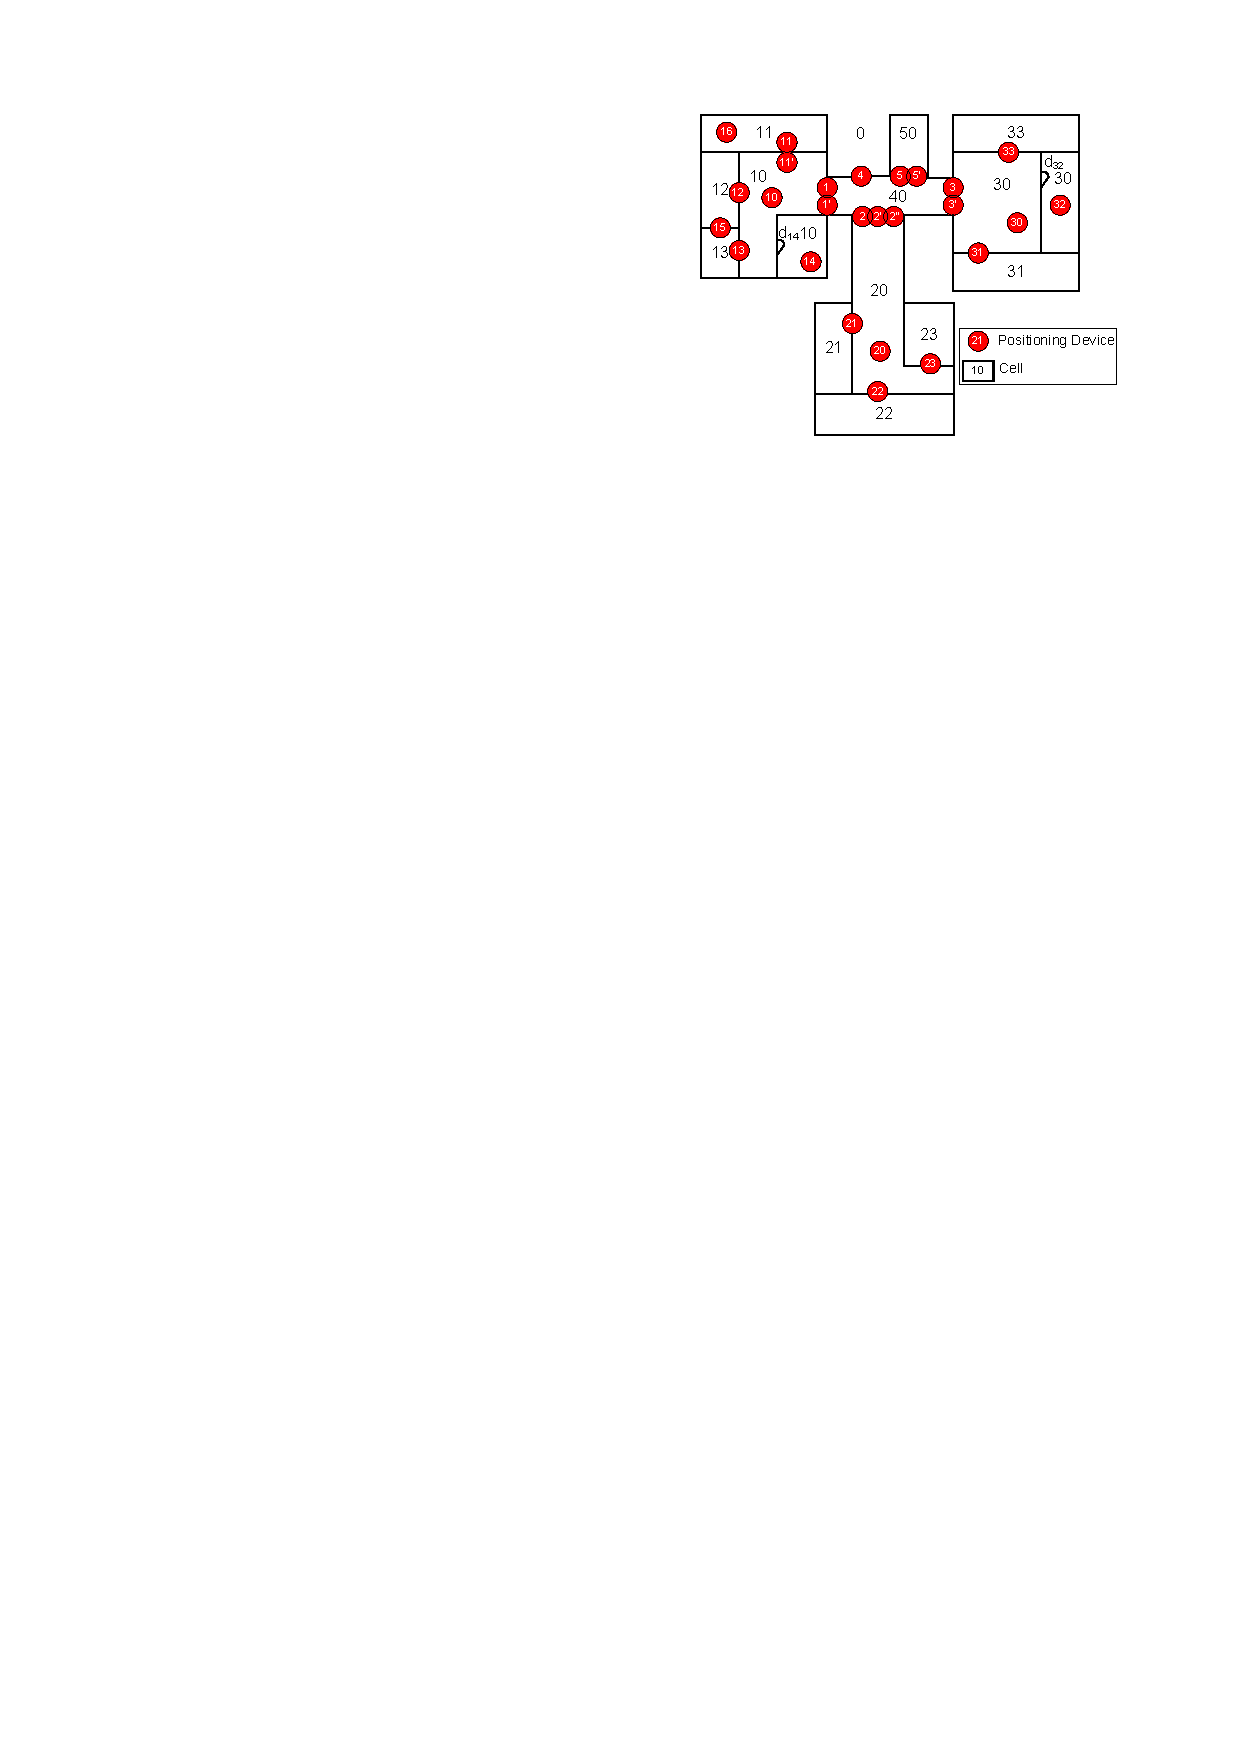
\includegraphics[width=\columnwidth]{figures/2-3/2-3-4.pdf}
    \end{figure}
    \vspace{-20pt}
    \pause
    \begin{figure}[tb]
      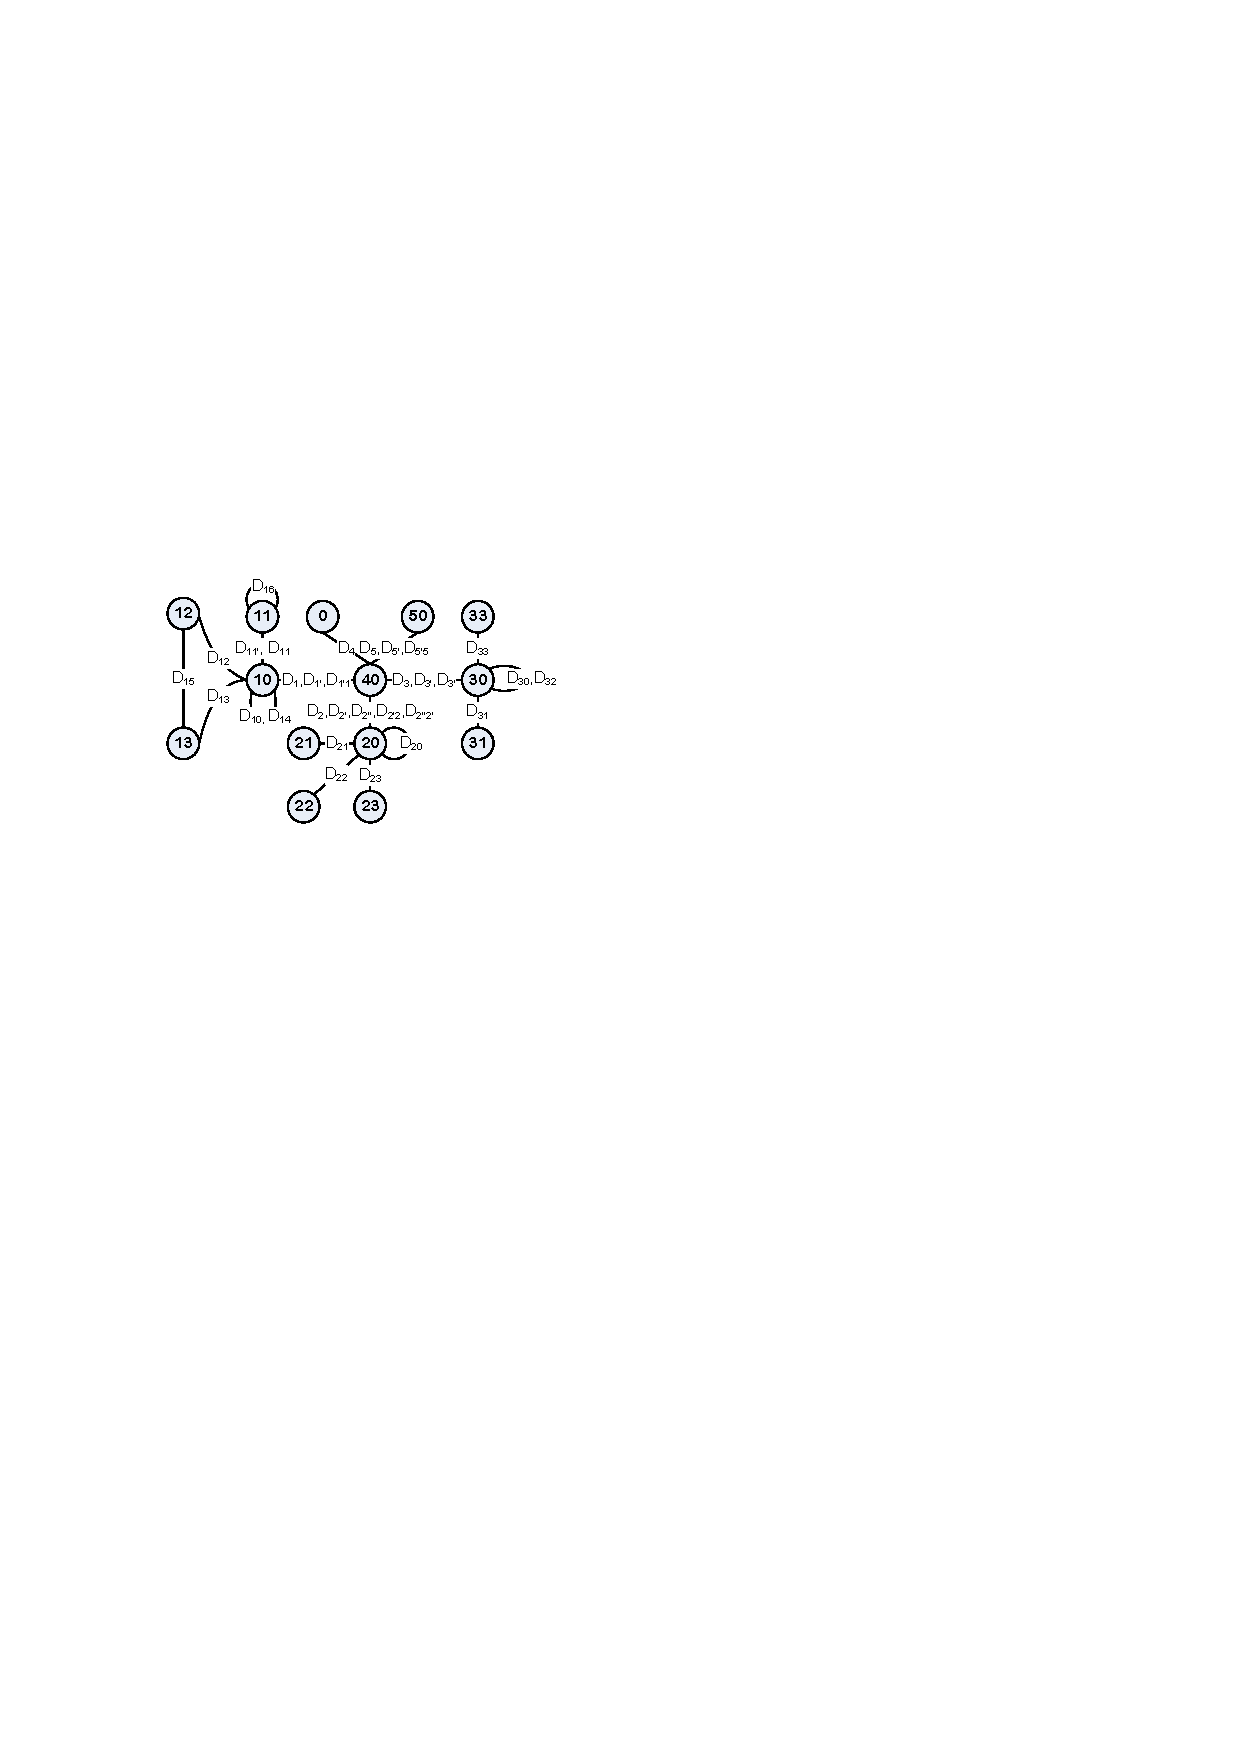
\includegraphics[width=\columnwidth]{figures/2-3/2-3-5.pdf}
    \end{figure}

\end{columns}

\end{frame}

%------------------------------------------------

\begin{frame}
\frametitle{States of Indoor Moving Objects~\cite{DBLP:conf/cikm/YangLJ09}}

%\begin{columns}[c]

  %\column{.57\textwidth}
  \begin{figure}[tb]
    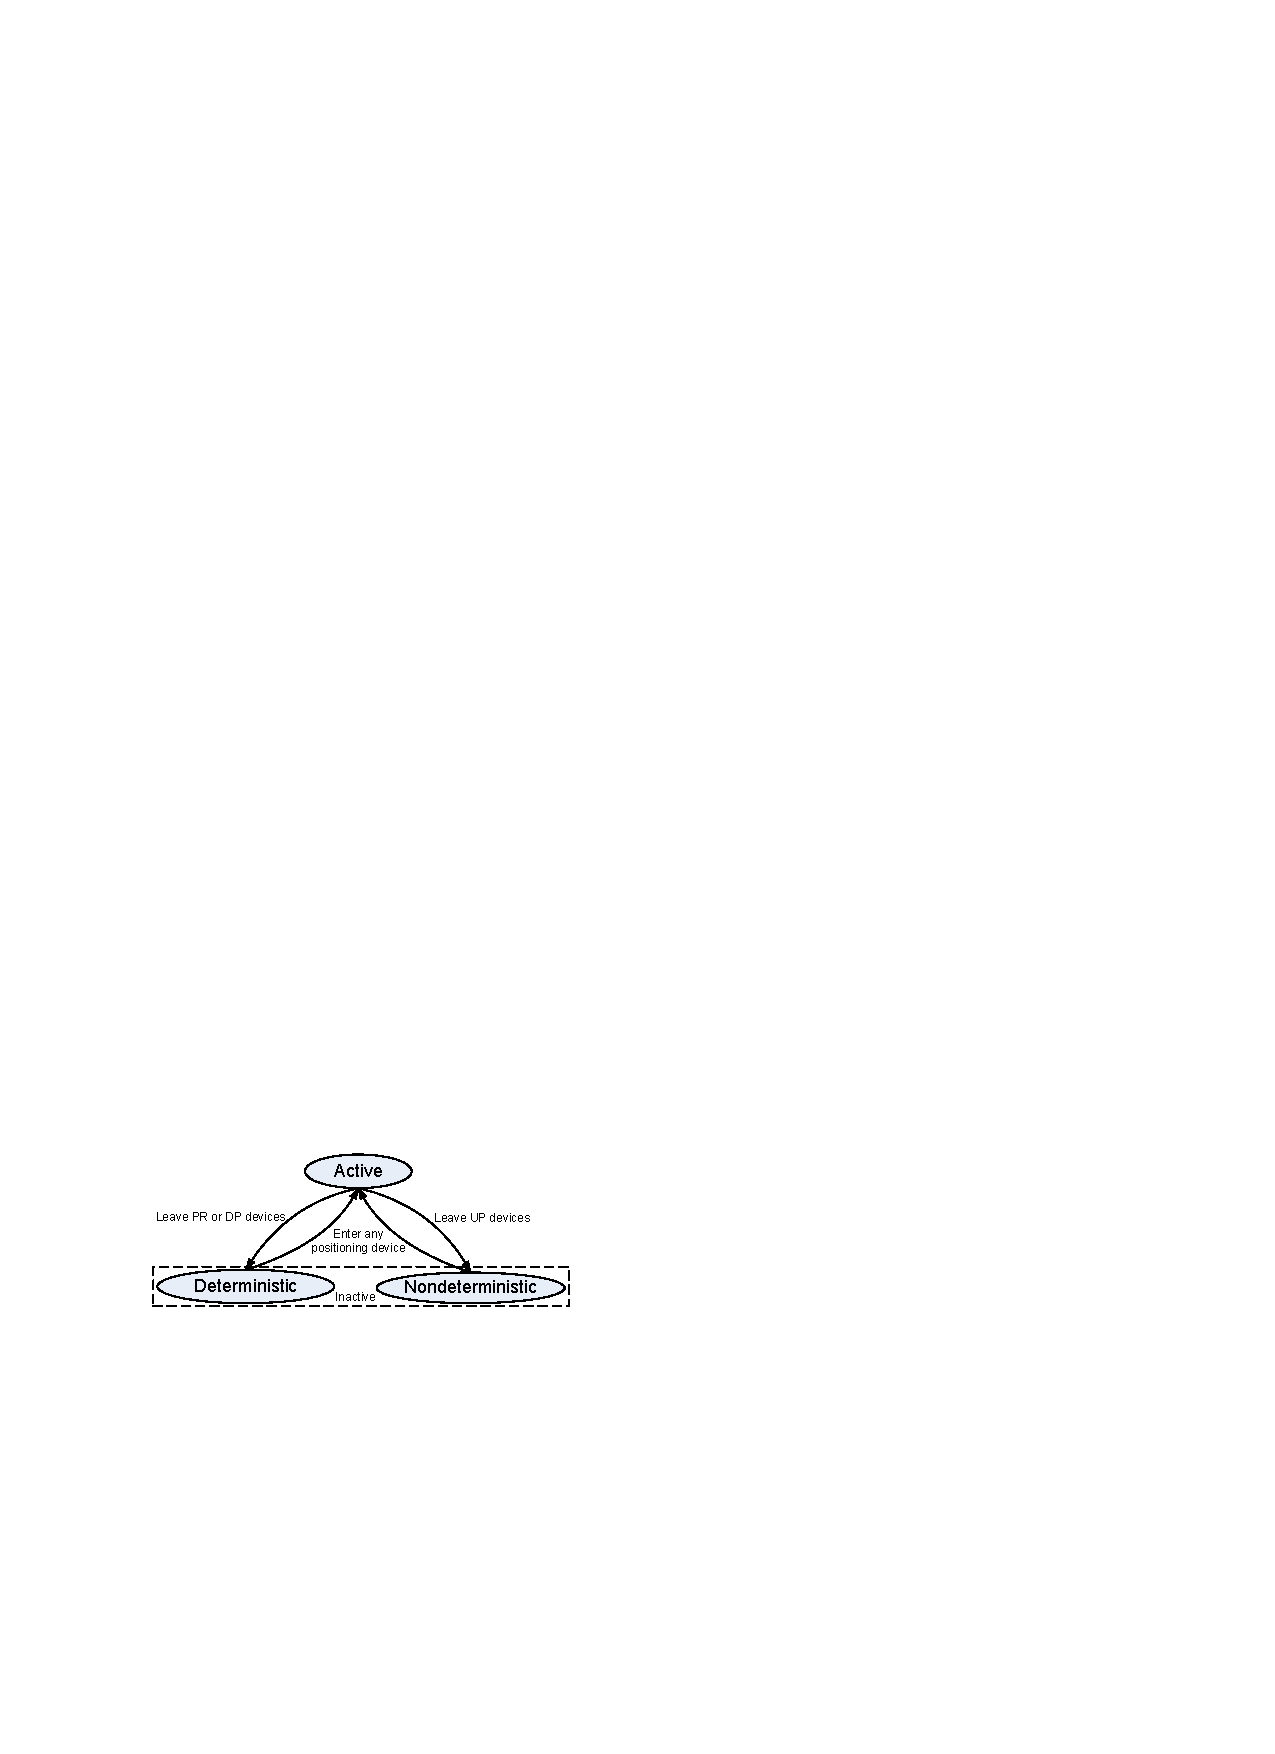
\includegraphics[width=0.6\columnwidth]{figures/2-2/2-2-3.pdf}
  \end{figure}
  \vspace{-10pt}
  %\column{.43\textwidth}
  \begin{itemize}
    \item An object is in an \conceptbf{active state} when it is inside the activation range of a positioning device.
    \item Otherwise the object is in an \conceptbf{inactive state}
    \item When an object is in the inactive state it is
      \begin{itemize}
        \item \conceptbf{nondeterministic} if it can be in more than one cell
        \item \conceptbf{deterministic} if it is in one specific cell
      \end{itemize}
  \end{itemize}

%\end{columns}

\end{frame}

%------------------------------------------------

\begin{frame}
\frametitle{Indexing Indoor Moving Objects~\cite{DBLP:conf/cikm/YangLJ09}}

\conceptbf{The proposed indexing scheme uses 4 hash tables}
\\~\\
\pause

\fsize{
\emph{Device Hash Table(DHT)} maps each device to a set of active objects:
\pause
$${DHT[deviceID] = O_A;~deviceID \in \Sigma_{devices}, O_A \subseteq O_{indoor}}$$
\\~\\
\pause

\emph{Cell Deterministic Hash Table(CDHT)} maps each cell to a set of deterministic objects:
\pause
$${CDHT[cellID] = O_D;~cellID \in C, O_D \subseteq O_{indoor}}$$
\\~\\
\pause

\emph{Cell Nondeterministic Hash Table(CNHT)} maps each cell to a set of nondeterministic objects:
\pause
$${CNHT[cellID] = O_N;~cellID \in C, O_N \subseteq O_{indoor}}$$
\\~\\
\pause

\emph{Object Hash Table(OHT)} maps objects to their current data(state, time, cell(s) the object can be in)
\pause
$${OHT[objectID] = (STATE, t, IDSet);~objectID \in O_{indoor}}$$
\\~\\
\pause
}

\end{frame}

%------------------------------------------------

\begin{frame}
\frametitle{RFID Deployment Graph Construction~\cite{DBLP:conf/cikm/YangLJ09}}

\begin{columns}[c]

  \column{.47\textwidth}
    \begin{figure}[tb]
      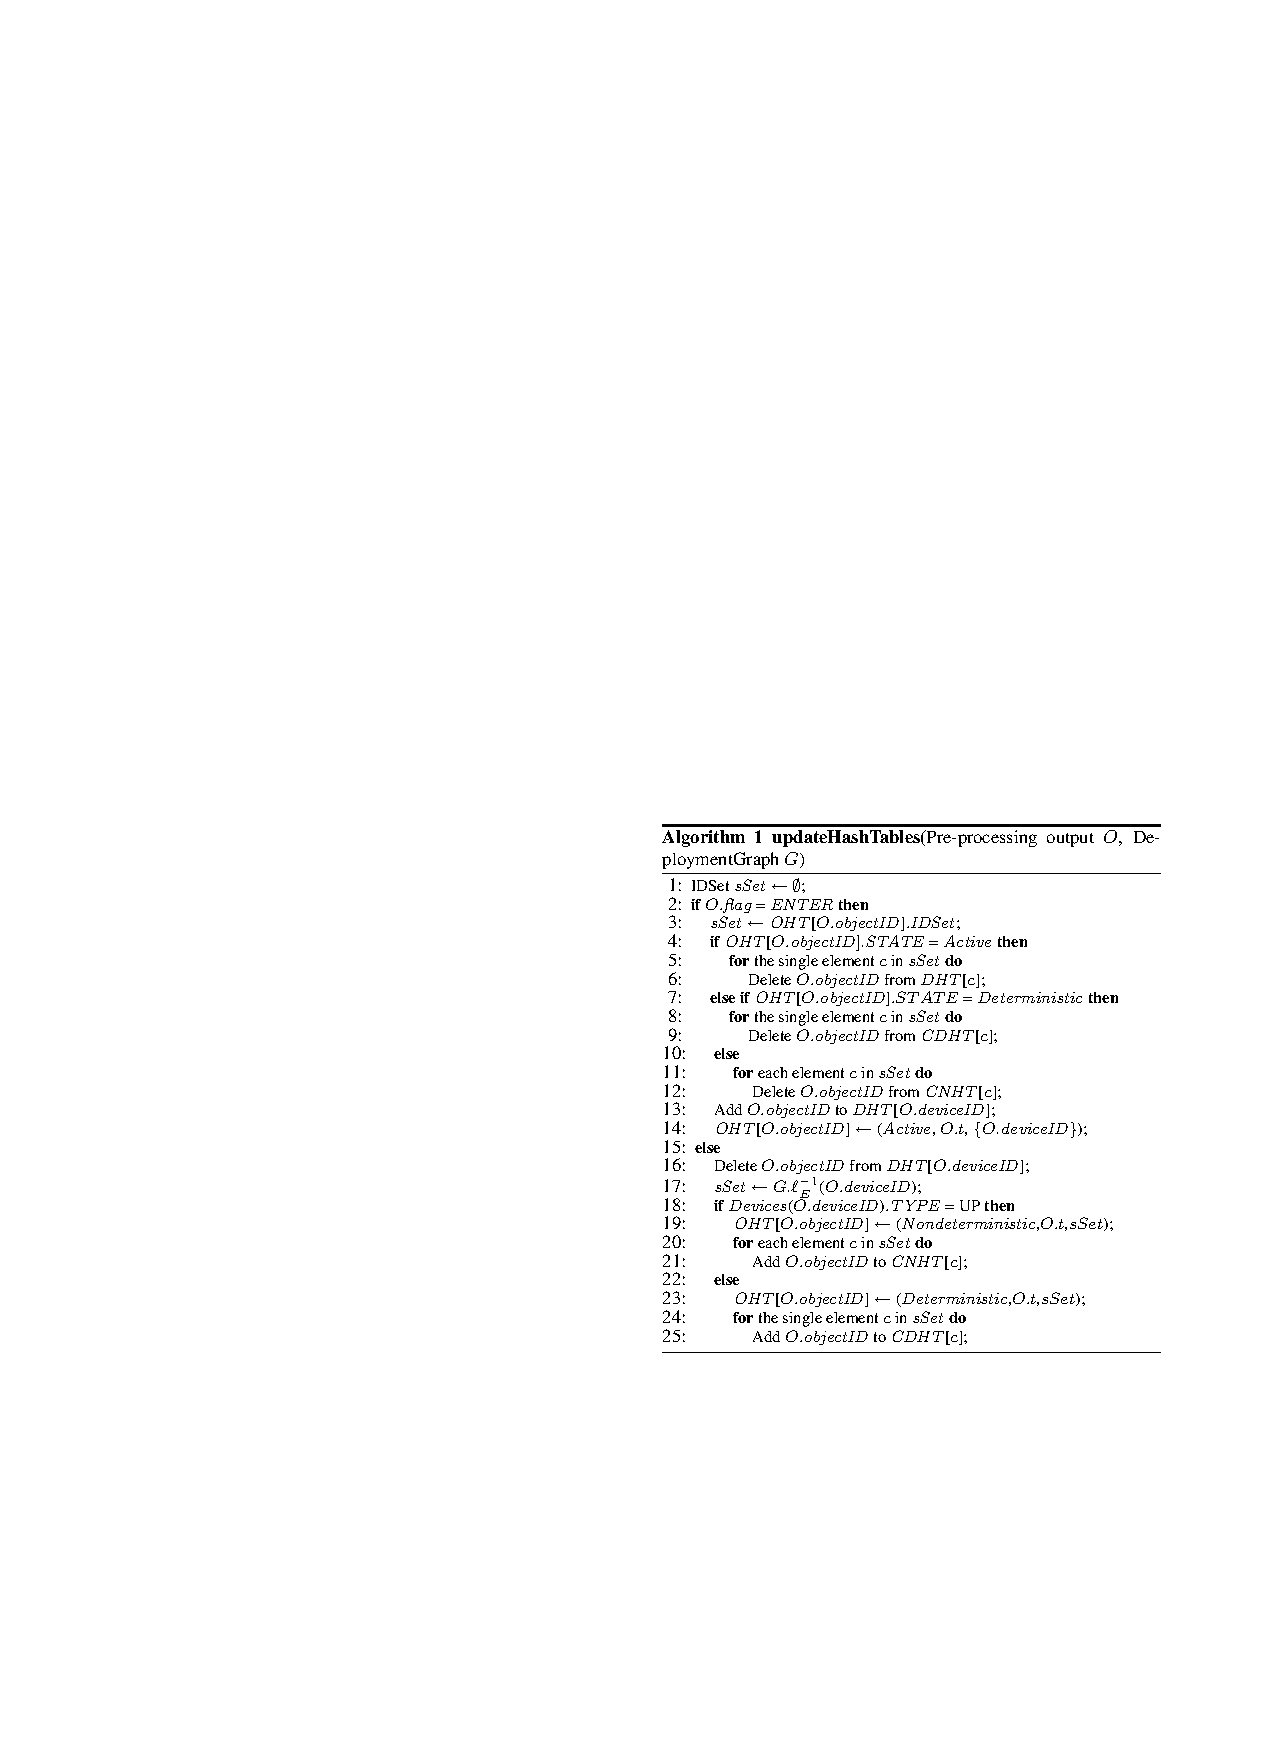
\includegraphics[width=\columnwidth]{figures/2-2/2-2-4.pdf}
    \end{figure}

  \column{.53\textwidth}
  \ssize{
    \begin{enumerate}
      \pause
      \item Line 1: \textrm{reset ${IDSet}$} \pause
      \item Lines 2--12: \textrm{${O.flag}$ is ENTER so check the object's previous state. Remove ${O}$ from the corresponding table according its previous state} \pause
      \item Lines 13--14: \textrm{add ${O}$ to table of active objects (DHT), and update ${O}$'s in the objects' table (OHT)} \pause
      \item Lines 16--17: \textrm{${O.flag}$ is LEAVE so remove the object from DHT. Get the possible cells that ${O}$ can move to} \pause
      \item Lines 18--25: \textrm{if the device is undirected, set ${O}$ in OHT and add ${O}$ to CNHT for the cells in sSet, else apply the same to CDHT}
    \end{enumerate}
  }
  \end{columns}

\end{frame}

%------------------------------------------------

\begin{frame}
\frametitle{Deriving Uncertain Regions for Indoor Moving Objects}

\textrm{For outdoor moving objects~\cite{cheng2004querying}, \conceptbf{Uncertainty Region}, denoted by ${UR(o,t)}$, is a region such that ${o}$ must be in this region at time ${t}$.}\\~

In general terms, an object ${o_i}$'s location can be modeled as a random variable with a probability density function ${f_{o_i}(x,y,t)}$ that has non-zero values only in ${o_i}$'s uncertainty region ${UR(o_i, t)}$.

\begin{equation}
  {\int_{UR(o_i,t)} f_{o_i}(x,y,t) dx dy = 1}
\end{equation}

\end{frame}

%------------------------------------------------

\begin{frame}
\frametitle{Deriving Uncertain Regions for Indoor Moving Objects}

Assume that an \emph{indoor object} has the same probability to be located anywhere inside its uncertainty region:
\begin{equation}
  {f_{o_i}(x,y,t) = \frac{1}{Area(UR(o_i, t))}, ~~(x,y) \in UR(o_i, t)}
\end{equation}

\begin{fitemize}
  \item \textbf{Active object}: the activation range of the corresponding device.
  \item \textbf{Deterministic object}: the intersection between the object's cell and its \emph{maximum-speed constrained circle}.
  \item \textbf{Nondeterministic object}: the union of the intersection between each cell and the circle.
\end{fitemize}

\end{frame}

%------------------------------------------------

\begin{frame}
\frametitle{Maximum-speed Constrained Circle}

\begin{columns}[c]

  \column{.48\textwidth}
    \begin{figure}[tb]
      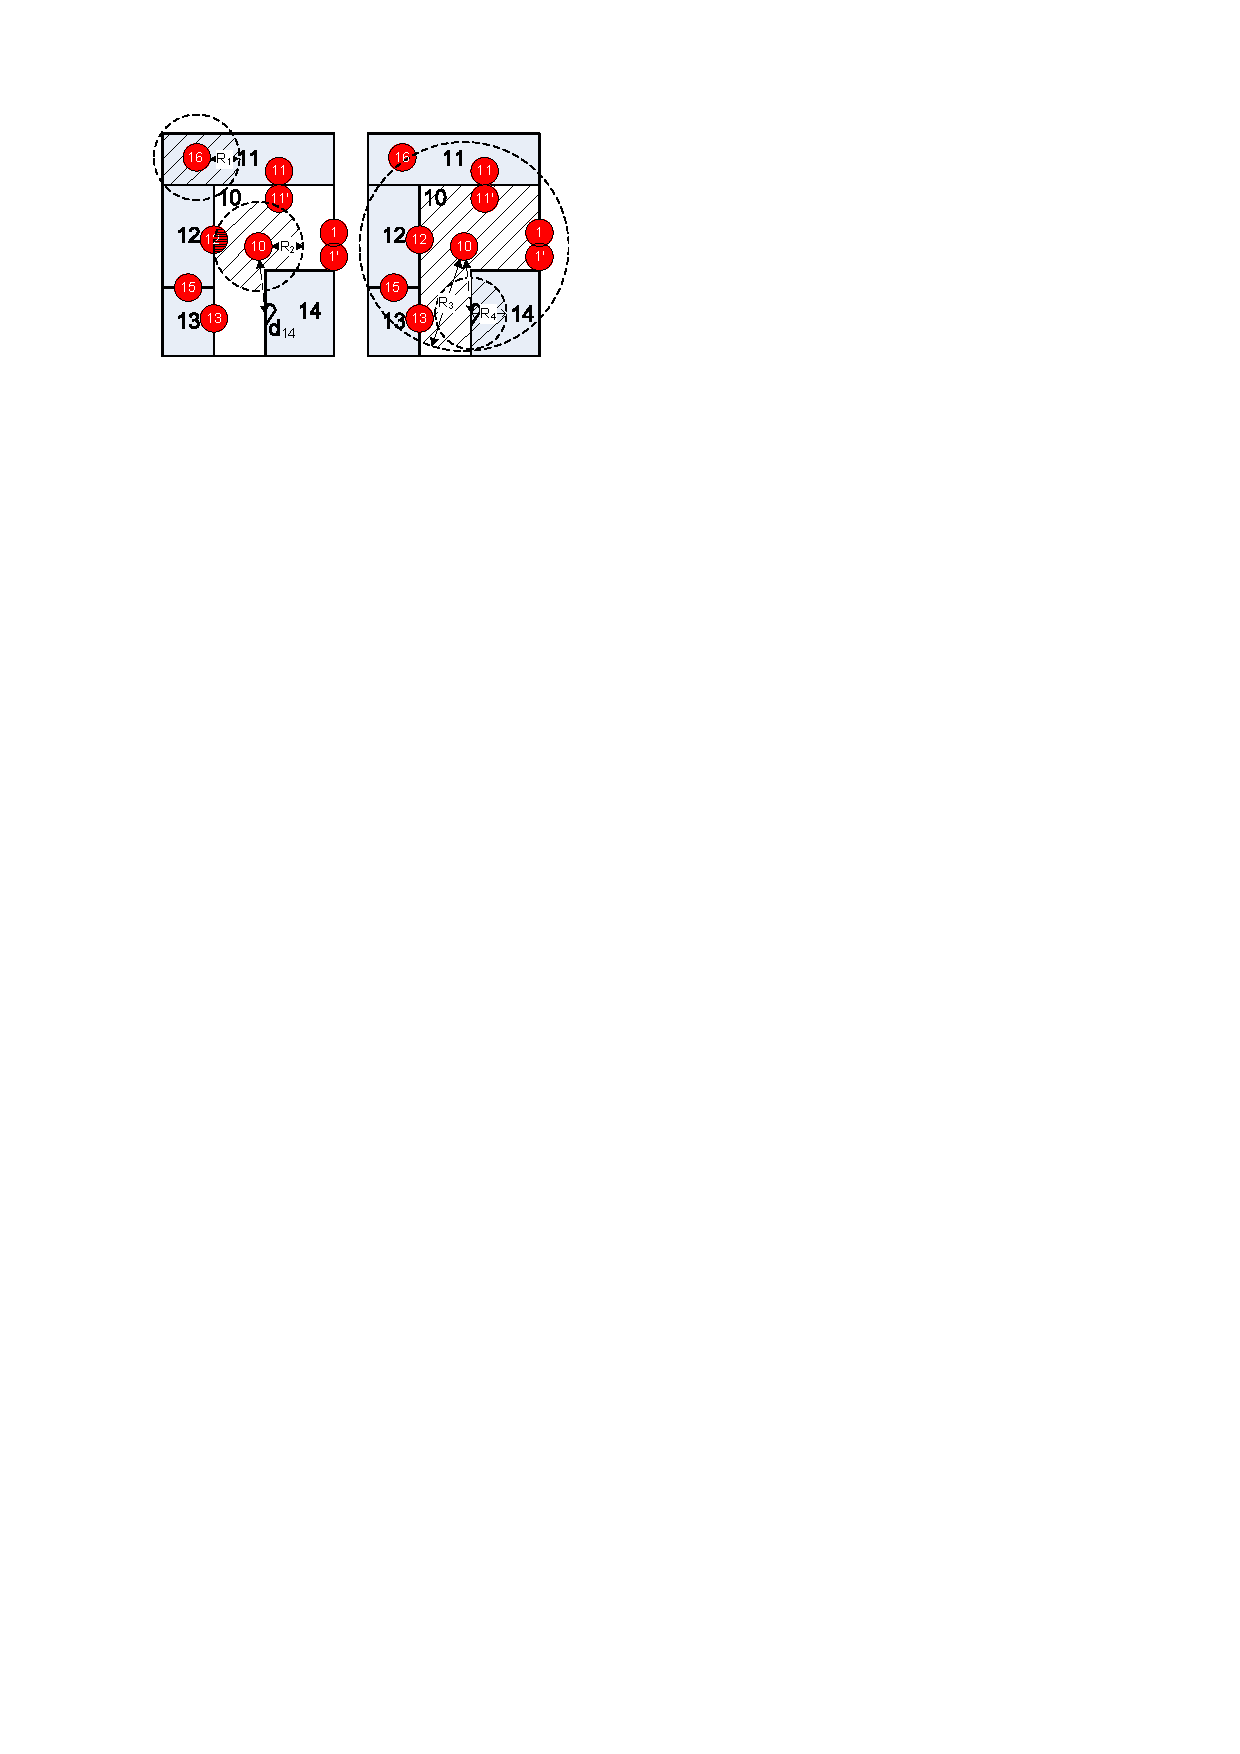
\includegraphics[width=\columnwidth,right]{figures/2-3/2-3-6.pdf}
    \end{figure}

  \column{.58\textwidth}
  \begin{fitemize}
      \item assume ${o}$ left ${device_{16}}$ at time ${t}$, intersection of maximum-speed constrained circle ${C_{MSC}(o, device_{16}, t)}$ and cell ${c_{11}}$.
      \item suppose ${o}$ left ${device_{10}}$ at time ${t}$, ${UR}$ is the intersection between room 10 and ${C_{MSC}(o, device_{10}, t)}$.
    \end{fitemize}

\end{columns}

\begin{fitemize}
  \item as time ${t}$ passes by, ${UR}$ therefore contains two parts...
  \item uncertainty region of an active object can be refined as the intersection of the activation range of device and ${C_{MSC}}$. suppose ${o}$ left ${device_{10}}$ and then is detected by ${device_{12}}$, its uncertainty region is the intersection of ${C_{MSC}(o, device_{10}, t)}$ and activation range of ${device_{12}}$.
\end{fitemize}

\end{frame}

%------------------------------------------------

\begin{frame}
\frametitle{PT$k$NN Query Processing}

\begin{definition}[Indoor Probabilistic Threshold $k$NN Query]
  \label{ptknnquery}
  \textrm{Given a set of indoor moving objects ${O = \{ o_1, o_2,...,o_n \}}$ and a threshold value ${T \in (0,1]}$, a PT${k}$NN query issued at time ${t}$ with query location ${q}$ returns a result set $\mathbb{R} = {\{ A | A \subseteq O \wedge |A| = k \wedge prob(A) > T \} }$, where ${prob(A)}$ is the probability that ${A}$ contains the ${k}$ nearest neighbors of the query location ${q}$ at time ${t}$.}
\end{definition}

~\\~
\small{when the number of moving objects increases, the number of ${k}$-subsets (${A}$ in Definition~\ref{ptknnquery}) in the result set $\mathbb{R}$ increase exponentially. Specifically, there are ${\binom{n}{k}}$ possible ${k}$-subsets for a PT${k}$NN query over ${n}$ objects.}

\end{frame}

%------------------------------------------------

\begin{frame}
\frametitle{PT$k$NN Query Processing}

\large{Three techniques are proposed to speed up PT$k$NN query processing:}
\begin{enumerate}
  \item minimum indoor walking distances between the query location and the (uncertainty regions of) objects are used to prune the objects too far away to be in any possible ${k}$-subset, results in a subset ${O' \subseteq O}$.
  \item for all ${k}$-subsets of ${O'}$, cost-efficient probability estimates are used to prune the ${k}$-subsets whose probabilities definitely are lower than the threshold ${T}$.
  \item for each remaining ${k}$-subset ${A}$, add ${A}$ to $\mathbb{R}$ only if ${prob(A) > T}$.
\end{enumerate}

\end{frame}

%------------------------------------------------

\begin{frame}
\frametitle{PT$k$NN Query Processing}

\footnotesize{
%Define the minimum and maximum MIWD between q and an uncertain object ${o_i}$.
Let ${s_i (l_i)}$ be the minimum(maximum) MIWD from q to the uncertainty region of ${o_i}$:
\pause
\begin{equation}
  {s_i = \min_{p \in UR(o_i,t)} d_{MIW}(q, p);~~~~l_i = \max_{p \in UR(o_i,t)} d_{MIW}(q, p)}
\end{equation}
}

\begin{columns}[c]

\column{.54\textwidth}
\begin{figure}[tb]
  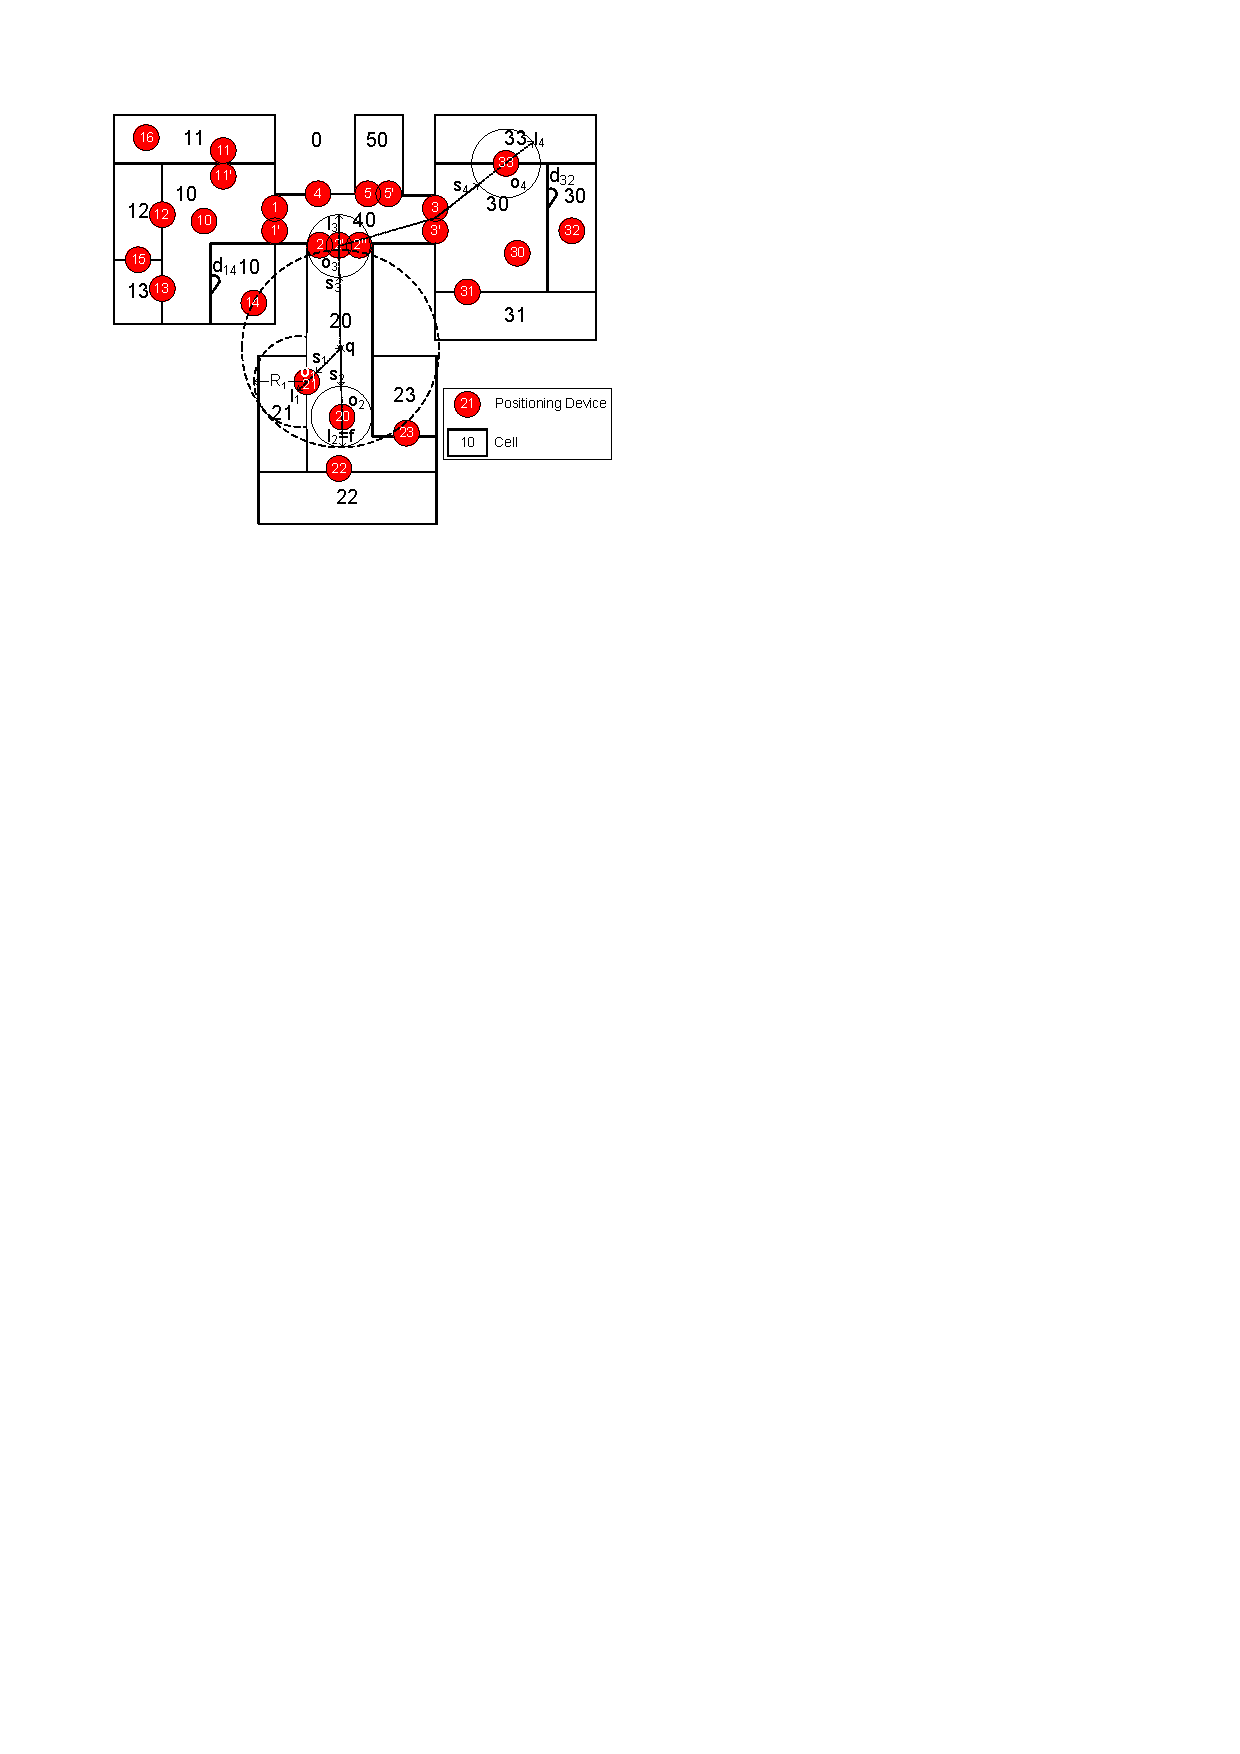
\includegraphics[width=\columnwidth]{figures/2-3/2-3-8.pdf}
\end{figure}

\column{.46\textwidth}
\begin{fitemize}
  \item ${o_1}$ is being observed by ${device_{12}}$
  \item ${o_2, o_3, o_4}$ recently left ${device_{20}, device_{2'}, device_{33}}$ respectively
  \item ${o_4}$'s MIWD computation should take into account the door connectivity
\end{fitemize}

\end{columns}

\end{frame}

%------------------------------------------------

\begin{frame}
\frametitle{PT$k$NN Query Processing}

\begin{definition}[k-bound]
  \textrm{Let ${f}$ be the ${k}$th minimal one of all objects' ${l_i}$s. If ${s_i}$ of object ${o_i}$ is greater than ${f}$, object ${o_i}$ has no chance to be in any ${k}$-subset of the result set $\mathbb{R}$. This ${f}$ value is called the k-bound.~\cite{cheng2009evaluating}}
\end{definition}

~\\
\begin{itemize}
  \item k-bound can be calculated and updated dynamically during the distance based pruning as soon as $k$ objects have been seen from ${O}$.
  \item by taking advantage of indoor space distance definition, the computation cost can be further reduced. E.g., the objects in the same cell can be pruned if one is pruned by the k-bound.
\end{itemize}

\end{frame}

%------------------------------------------------

\begin{frame}
\frametitle{Distance Pruning}

\begin{columns}[c]

  \column{.47\textwidth}
    \begin{figure}[tb]
      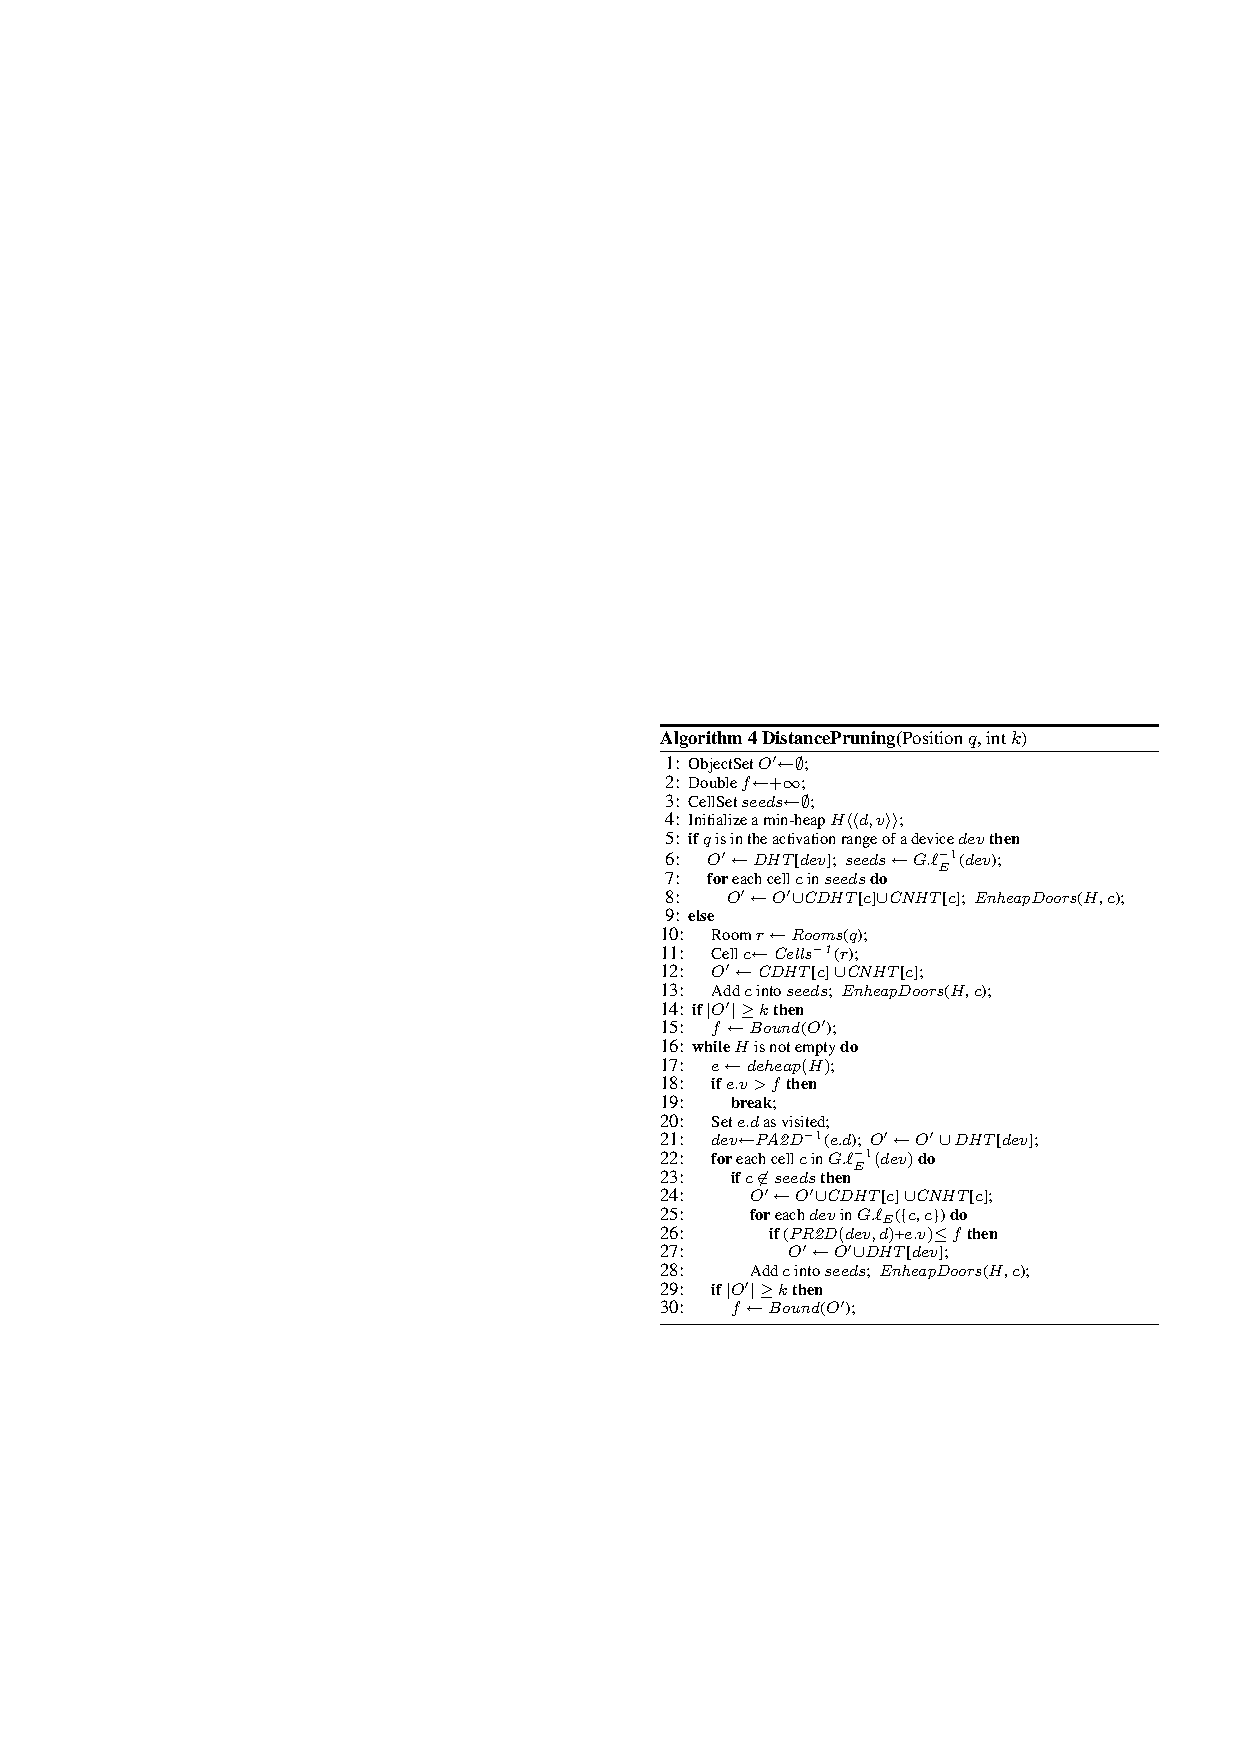
\includegraphics[width=\columnwidth]{figures/2-3/2-3-9.pdf}
    \end{figure}

  \column{.53\textwidth}
  \ssize{
    \begin{enumerate}
      \pause
      \item Lines 1--4: \textrm{initialization: candidate object set ${O'}$, k-bound ${f}$, cell set ${seeds}$ records the examined cells, min-heap ${H \langle \langle d, v \rangle \rangle}$ gives priority to doors closer to location ${q}$} \pause
      \item Lines 5--8: \textrm{if ${q}$ is in ${dev}$'s activation range, active objects in ${dev}$ are added to ${O'}$, the nearby objects are added are also added to ${O'}$} \pause
      \item Lines 9--13: \textrm{if not, the covering cell ${c}$ is added to set ${seeds}$, add both deterministic and nondeterministic objects to ${O'}$} \pause
      \item Lines 14--15: \textrm{determine the k-bound from the current ${O'}$} \pause
      \item Lines 17-30: \textrm{expansion step followed Dijkstra, stops when the entry's distance is too far away, if ${|O'|>k}$ then update ${f}$ and reduce the candidate set ${O'}$} \pause
    \end{enumerate}
  }
  \end{columns}

\end{frame}

%------------------------------------------------

\begin{frame}
\frametitle{Probability Threshold Based Pruning}

\textit{\textrm{There can still be ${\binom{|O'|}{k}}$ possible ${k}$-subsets in result set $\mathbb{R}$.}}
\\~\\
\ssize{
  \pause
  Given an object ${o_i}$, let ${P_{o_i}(r)}$ be the cumulative distribution function that ${o_i}$'s MIWD to the query location ${q}$ is ${r}$:
  \pause
  \begin{equation}
    { P_{o_i}(r) = Pr(d_{MIW}(q, o_i) \leq r) }
  \end{equation}
  ~\\
  Let ${A}$ be a ${k}$-subset of ${O'}$. The probability ${Prob(A)}$ that ${A}$ contains the ${k}$ nearest neighbors of ${q}$ satisfies:
  \pause
  \begin{equation}
    { Prob(A) \leq \prod_{o_i \in A} P_{o_i}(f) }
  \end{equation}
  ~\\
  If ${P_{o_i}(f)}$ is less than the threshold ${T}$, any ${k}$-subset ${A}$ that contains ${o_i}$ satisfies:
  \pause
  \begin{equation}
    { Prob(A) \leq \prod_{o_i \in A} P_{o_i}(f) \leq P_{o_i}(f) \leq T }
  \end{equation}
  Therefore, if ${P_{o_i}(f) \leq T}$, ${o_i}$ can be safely pruned from the candidate.
}

\end{frame}

%------------------------------------------------

\begin{frame}
\frametitle{Probability Evaluation}

\textit{\textrm{After probability threshold pruning, each ${k}$-subset ${A}$ in $\mathbb{R}$ may have their ${Prob(A)}$ greater than ${T}$.}}
\\~\\
\ssize{
Define ${Prob(A)}$ as:
\pause
\begin{equation}
  { Prob(A) = \sum_{o_z \in A} \int_{0}^{+\infty}p_{o_z}(r) \prod_{o_i \in A \setminus \{ o_z\}} P_{o_i}(r) \prod_{o_j \in O' \setminus A} (1 - P_{o_j}(r)) dr}
\end{equation}
\pause
}
\begin{columns}[c]

  \column{.42\textwidth}
    \begin{figure}[tb]
      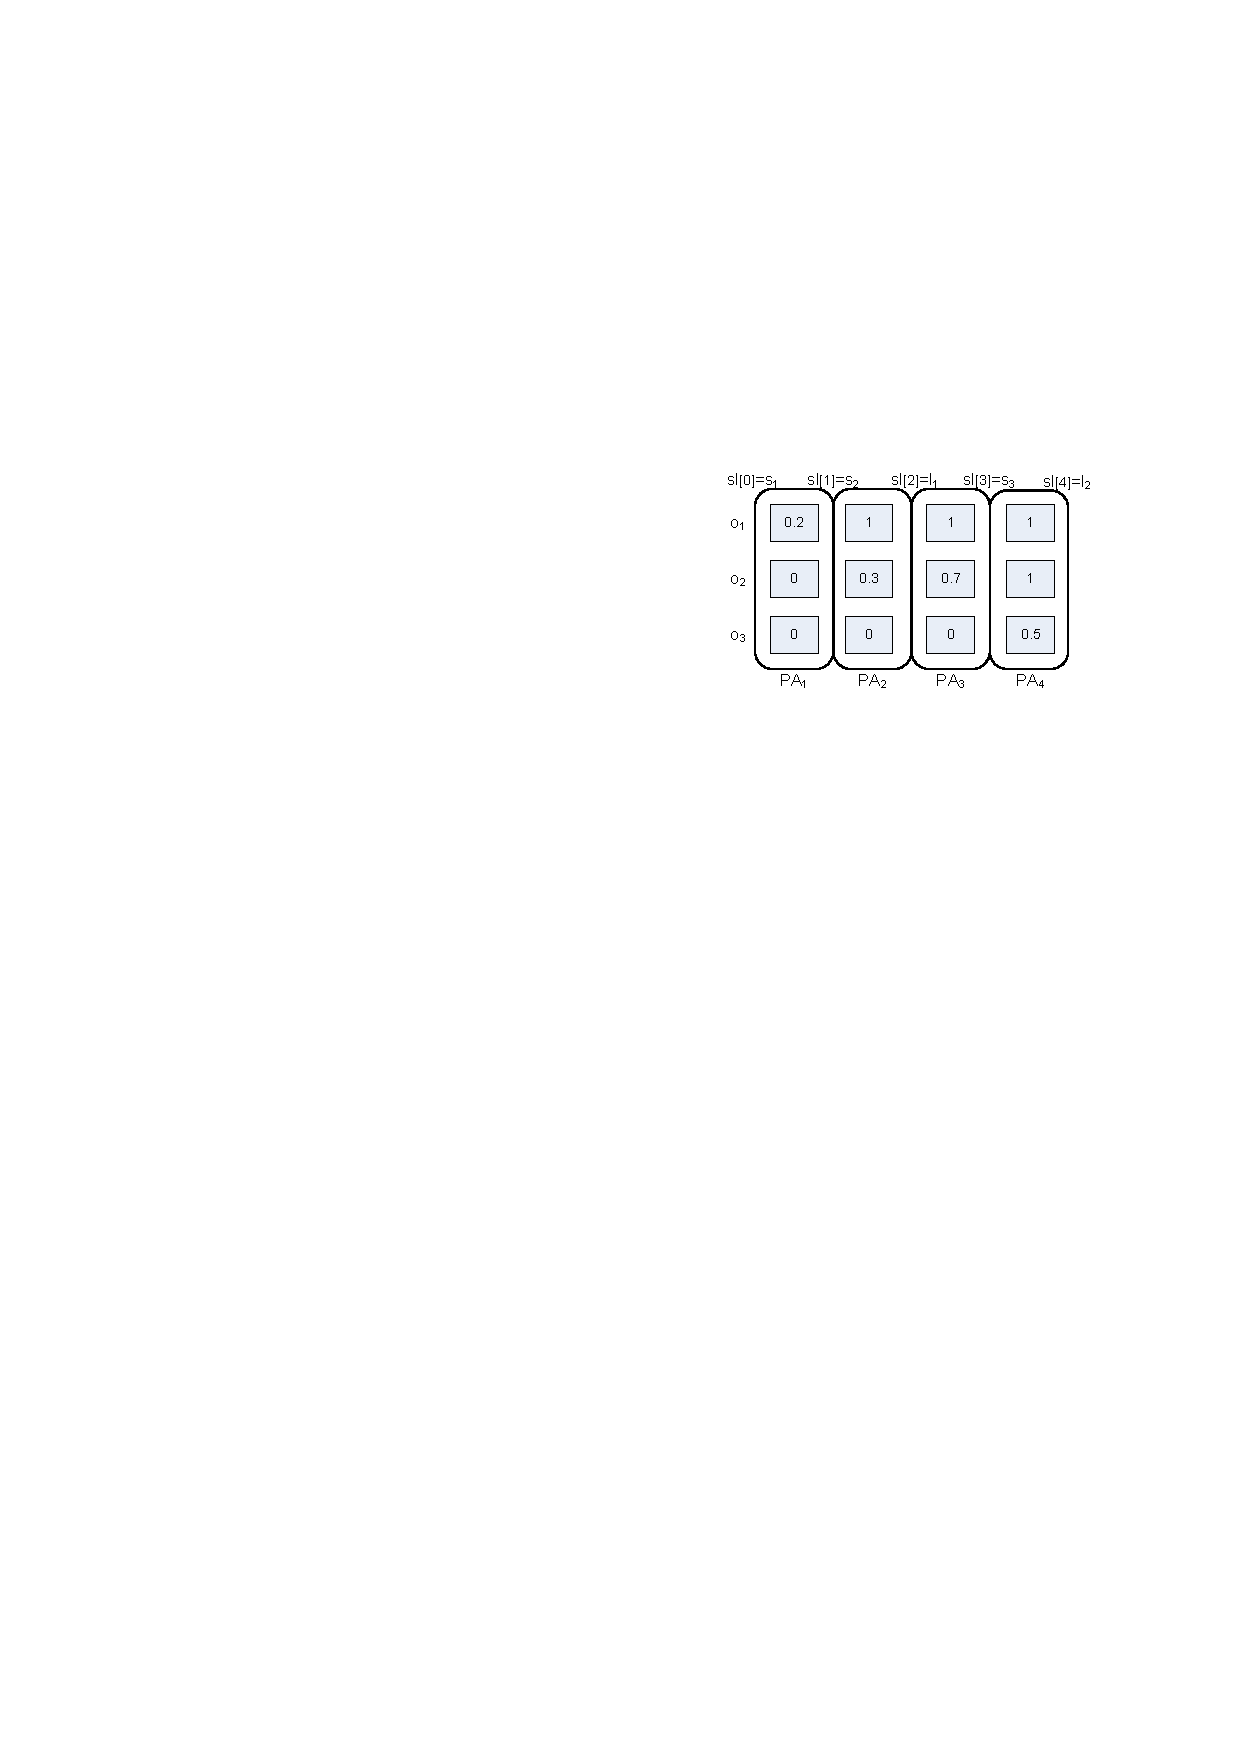
\includegraphics[width=\columnwidth]{figures/2-3/2-3-10.pdf}
    \end{figure}

  \column{.58\textwidth}
  \begin{sitemize}
    \item ${o_z}$ is the ${k}$-th nearest neighbor of ${q}$.
    \item to evaluate the probabilities efficiently, a partition based approximate evaluation method is used.
    \item let an array ${sl}$ records all the minimum distances ${s_i}$ in ${O'}$ and the maximum distances ${l_i}$ that satisfy ${l_i \leq f}$.
    \item ${sl}$ should have ${g = |O'| + k}$ elements, sort it in ascending order.
  \end{sitemize}
\end{columns}

\end{frame}

%------------------------------------------------

\begin{frame}
\frametitle{Research Directions}

\begin{itemize}
  \item Analyzing historical trajectory data may discover associations among object movements, which can be used to design more efficient group pruning in processing a PT${k}$NN query
  \\~\\
  \item Regarding the uncertainty model of indoor moving objects, it is also interesting to conduct probabilistic analysis on other kinds of object distribution.
\end{itemize}

\end{frame}
